\documentclass[11pt,a4paper]{article}

% These are extra packages that you might need for writing the equations:
\usepackage{amsmath}
\usepackage{amsfonts}
\usepackage{amssymb}
\usepackage{booktabs}
\usepackage{hyperref}
\usepackage{listings}
\usepackage{xcolor}
\usepackage{outlines}
\usepackage{mathtools}



\lstset {language=C++,
		 basicstyle=\ttfamily,
         keywordstyle=\color{blue}\ttfamily,
         stringstyle=\color{red}\ttfamily,
         commentstyle=\color{purple}\ttfamily,
         morecomment=[l][\color{magenta}]{\#},
       	 basicstyle=\tiny}

% You need the following package in order to include figures in your report:
\usepackage{graphicx}

% With this package you can set the size of the margins manually:
\usepackage[left=2cm,right=2cm,top=2cm,bottom=2cm]{geometry}

\renewcommand{\vec}[1]{\mathbf{#1}}
\newcommand{\norm}[1]{\left\lVert#1\right\rVert}

\begin{document}

% Enter the exercise number, your name and date here:
\noindent\parbox{\linewidth}{
 \parbox{.25\linewidth}{ \large ICP, Exercise 11 }\hfill
 \parbox{.5\linewidth}{\begin{center} \large Beat Hubmann \end{center}}\hfill
 \parbox{.2\linewidth}{\begin{flushright} \large Dec 07, 2018 \end{flushright}}
}
\noindent\rule{\linewidth}{2pt}


\section{Introduction}

The Jacobi relaxation method and the Gauss-Seidel method were implemented to solve
the discretized Poisson equation in two dimensions for point charges in a grounded box.
The two methods were compared with each other in terms of time to solution and number of iterations required.
Also, the time to solution was compared to a high performance library Cholesky solver.

\section{Algorithm Description}

For all cases, the two-dimensional Poisson equation(equation~\ref{eqn:1}) on $\Omega$ is 
discretized using second-order central finite differences in both the x- and the y-direction (equation~\ref{eqn:2}).
Both axes share a common grid spacing of $\Delta x= \frac{1}{N+1}$ where $N$ is the number of interior points
per axis direction on the grid.
Following the established finite difference method procedure to employ natural ordering, the left-hand side of equation~\ref{eqn:2} then can be written
in form of an $N*N \times N*N$ matrix $\vec{A}$ while the values of $\phi$ on the grid get unrolled into a vector $\vec{b}$ of size $N*N$ on the right-hand side (equation~\ref{eqn:3}).\\
The resulting matrix $A$ is both sparse and block tridiagonal.



\begin{equation}
\Delta \Phi = -\phi \quad \text{on}\ \Omega = (0, 1) \times (0,1)
\label{eqn:1}
\end{equation}


\begin{equation}
4x_{i,j} - x_{i-1, j} - x_{x+1, j} - x_{i, j-1} - x_{i, j+1} = -(\Delta x)^2 \cdot \rho(x_{i,j})
\label{eqn:2}
\end{equation}


\begin{equation}
Ax = b
\label{eqn:3}
\end{equation}


\subsection{Jacobi relaxation method}
In matrix form, the Jacobi method works by decomposing the matrix $\vec{A}$ into a matrix $\vec{D}$ consisting only of $\vec{A}$'s main diagonal
and a remainder matrix $\vec{R} = \vec{A} - \vec{D}$. Starting with an initial guess for $\vec{x} = (1, 1, \ldots, 1)^{\text{T}}$, we iterate $\vec{x}^{(t+1)} = \vec{D}^{-1}(\vec{b}- \vec{R}\vec{x}^{(t)})$
until $\norm{\vec{x}^{(t+1)} - \vec{x}^{(t)}}$ becomes smaller than a chosen convergence treshold in a chosen norm.


\subsection{Gauss-Seidel method}
Similar to the Jacobi relaxation method, the matrix $\vec{A}$ is decomposed into a lower triagonal matrix $\vec{L}$ and a strictly upper triagonal matrix $\vec{U}$ such that
$\vec{A} = \vec{L} + \vec{U}$. Completely analogous to the Jacobi relaxation method, the iteration step is  $\vec{x}^{(t+1)} = \vec{L}^{-1}(\vec{b}- \vec{U}\vec{x}^{(t)})$.

\section{Results}

The program was implemented as described above and submitted with this report. \\
Both methods reached the set conversion treshold of $\norm{\vec{x}^{(t+1)} - \vec{x}^{(t)}}_{2} \le 10^{-4}$. \\
The Jacobi relaxation method took $t=3478$ iterations but on average only $\sim 45 \text{ms}$ to do so, while the Gauss-Seidel method
only took $t=1922$ iterations but $\sim 6400 \text{ms}$ to reach the same treshold. For comparison, Eigen's optimized library Cholesky method
solver obtained the reference solution in $9 \text{ms}$.\\
Both methods' solutions reached similar deviation from the reference Cholesky solution:\\ 
$\norm{\vec{x}^*_{\text{Jacobi}} - \vec{x}^*_{\text{Cholesky}}}_{2} \approxeq  \norm{\vec{x}^*_{\text{Gauss-Seidel}} - \vec{x}^*_{\text{Cholesky}}}_{2} \approxeq 0.05$.
The heat maps for all three solvers are shown in figures~\ref{fig:1}, \ref{fig:2} and~\ref{fig:3}.


\begin{figure}[ht]
\begin{center}
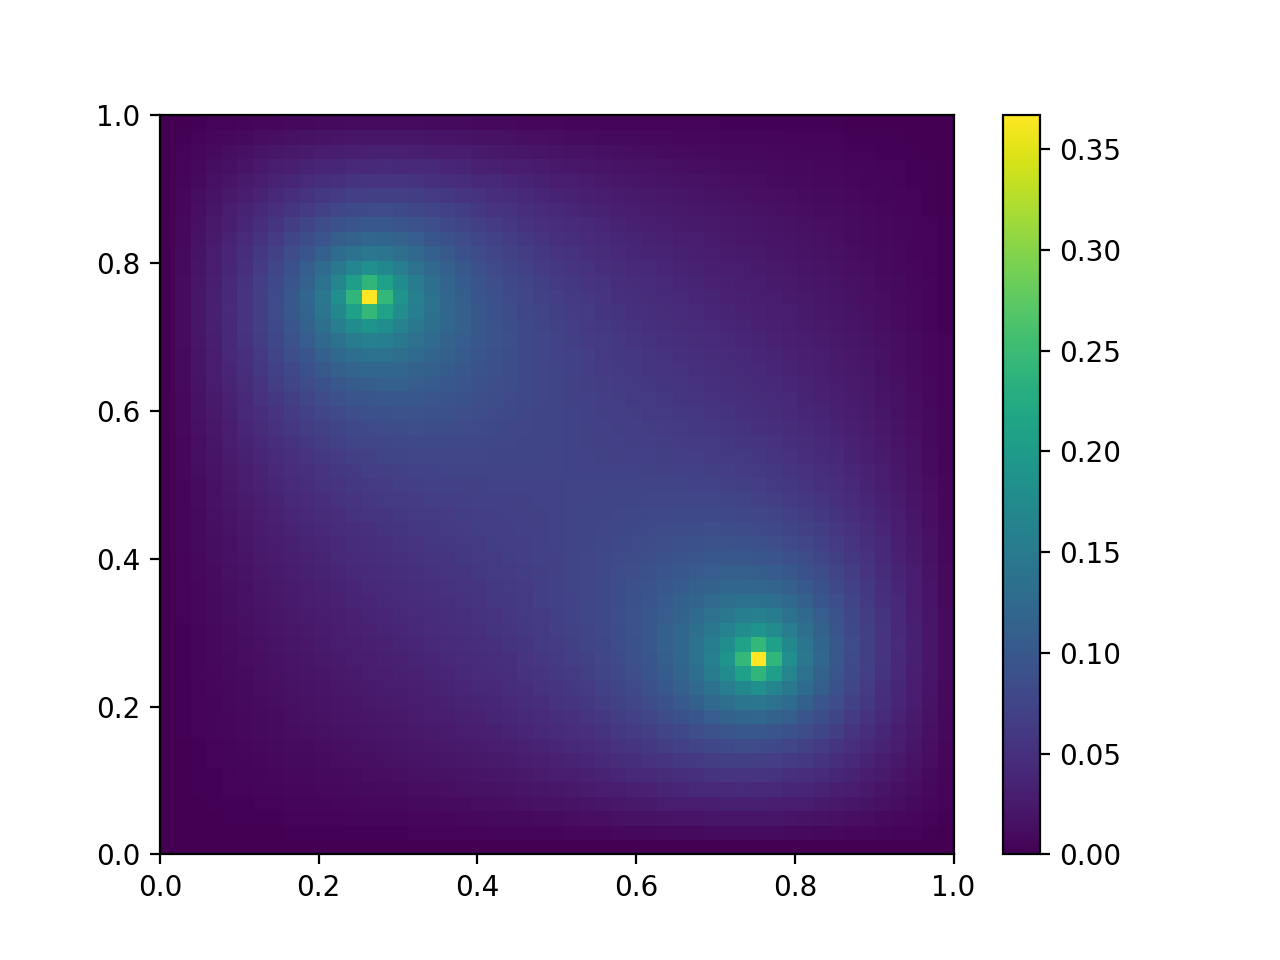
\includegraphics[scale=1.2]{figure_1.png} 
\end{center}
\caption{Cholesky solver reference solution for Poisson equation with point charges at $(0.25, 0.75)$, $(0.75, 0.25)$.}
\label{fig:1}
\end{figure}

\begin{figure}[ht]
\begin{center}
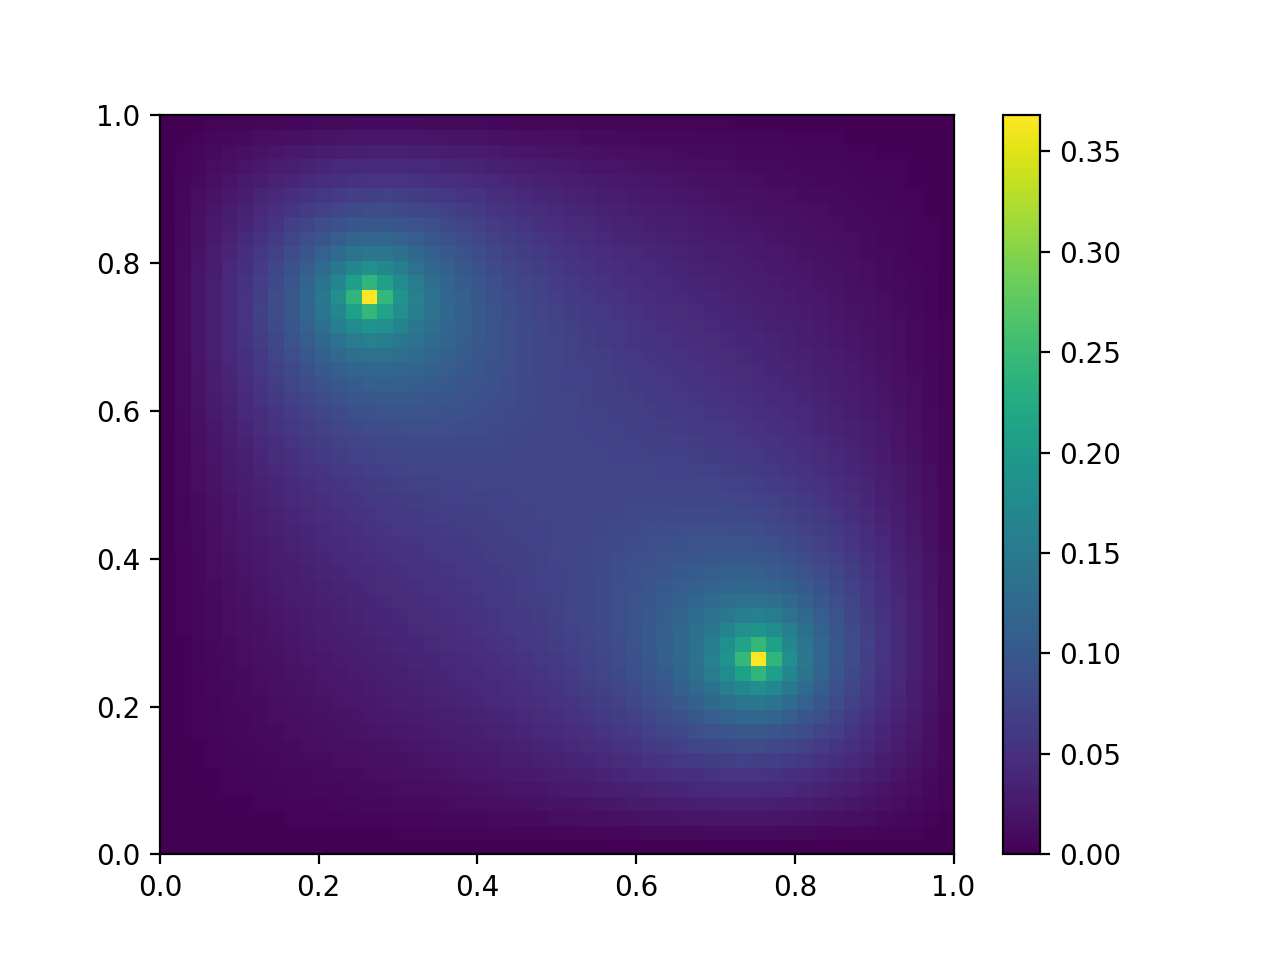
\includegraphics[scale=1.2]{figure_2.png} 
\end{center}
\caption{Jacobi relaxation solver solution for Poisson equation with point charges at $(0.25, 0.75)$, $(0.75, 0.25)$.}
\label{fig:2}
\end{figure}

\begin{figure}[ht]
\begin{center}
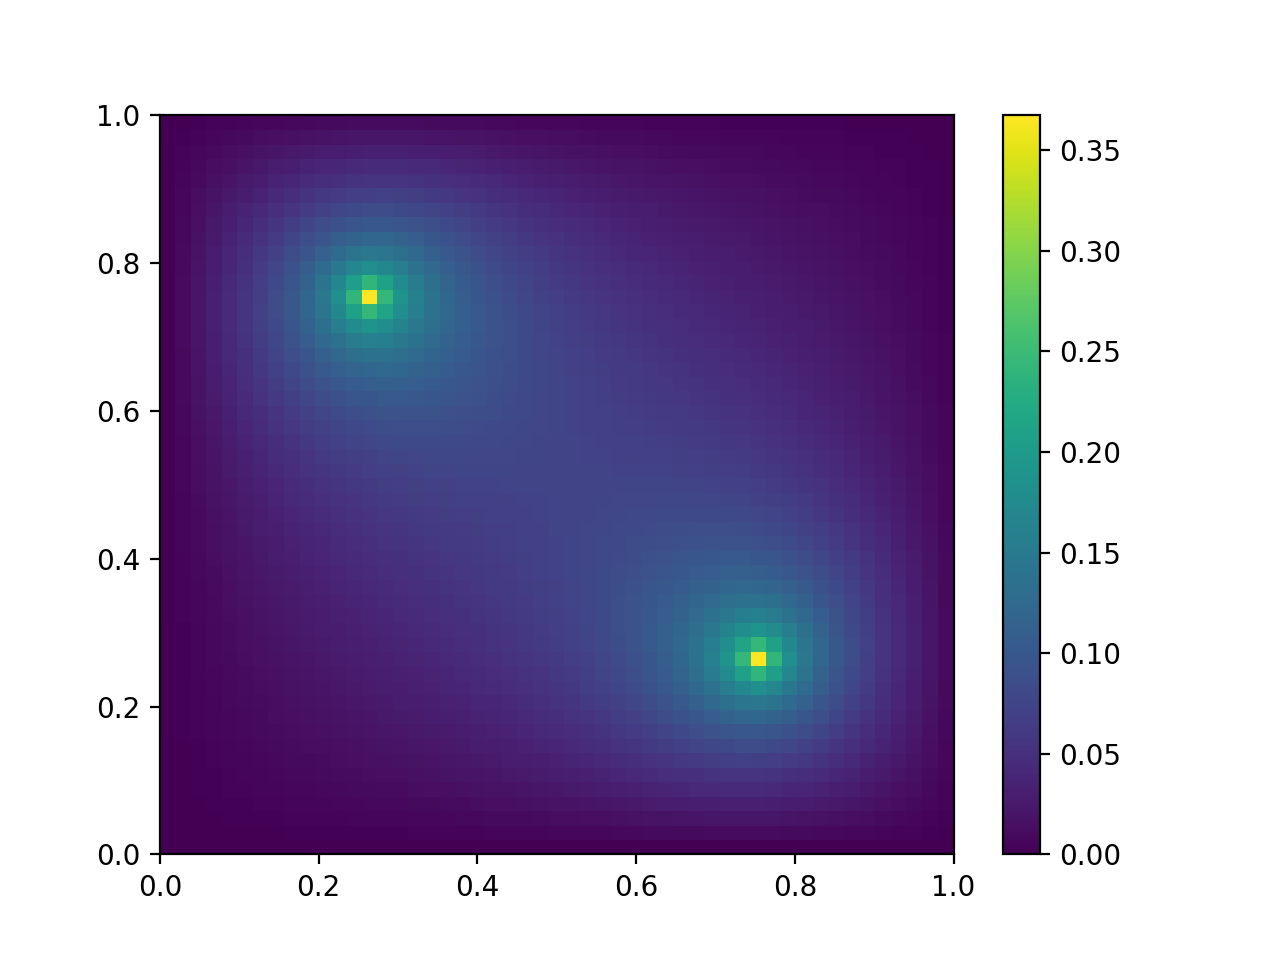
\includegraphics[scale=1.2]{figure_3.png} 
\end{center}
\caption{Gauss-Seidel solver solution for Poisson equation with point charges at $(0.25, 0.75)$, $(0.75, 0.25)$.}
\label{fig:3}
\end{figure}

\section{Discussion}
The results are as expected. Further consideration should be given to investigating why the Gauss-Seidel solver
in this implementation is an order of magnitude slower than the Jacobi relaxation solver.

%\begin{thebibliography}{99}


% \bibitem{metropolis}
% Metropolis, N.,
% Rosenbluth, A.W.,
% Rosenbluth, M.N.,
% Teller, A.H.,
% Teller, E.\\
% \emph{Equations of State Calculations by Fast Computing Machines},\\
% Journal of Chemical Physics. 21 (6): 1087,\\
% 1953.


% \bibitem{herrmann}
% 	Herrmann, H. J.,
% 	Singer, H. M.,
% 	Mueller L.,
% 	Buchmann, M.-A.,\\
% 	\emph{Introduction to Computational Physics - Lecture Notes},\\
% 	ETH Zurich,\\
% 	2017.

% \bibitem{Gottschling}
% Gottschling, Peter\\
% \emph{Discovering Modern C++},\\
% Addison-Wesley,\\
% 2016.




%\end{thebibliography}

\end{document}